\documentclass[12pt,a4paper,spanish]{article} 
\usepackage{babel}
\usepackage [T1]{fontenc}
\usepackage [latin1]{inputenc}
\usepackage{graphicx} 
\usepackage{array}
	  \oddsidemargin 0in
      \textwidth 6.75in
      \topmargin 0in
      \textheight 10.0in
      \parindent 0em
      \parskip 2ex
\usepackage{anysize}
\marginsize{3cm}{2cm}{1.0cm}{1.0cm}

\pagestyle{plain}

\begin{document} 
\title{
\begin{table}[!h]
	\begin{tabular}{m{2cm}m{15cm}}
		\multicolumn{1}{l}{}
		 
\includegraphics[scale=0.25, bb=0 0 0 0]{logo-fiuba.PNG} & 
		 \begin{center}
		 	\begin{LARGE}
				Universidad de Buenos Aires	\linebreak \linebreak		 							Facultad de Ingenier\'{i}a  \linebreak \linebreak
				7515 - Base de Datos \linebreak \linebreak
				1er. Cuatrimestre de 2010
			\end{LARGE}
		 \end{center}\\
\end{tabular}
\end{table}
\begin{Large}
 \begin{center}
		\underline{TP Base de Datos: SIGeek} \linebreak \linebreak
        Docente a cargo: Ing. Lucas Roman
\end{center}
\end{Large}
}
\date{}
\maketitle

\thispagestyle{empty}
\author{
\begin{Large}
\begin{center}
		\underline{Integrantes}  \linebreak 
\end{center}
\end{Large}
\begin{center}
	\begin{tabular}{|| c | c | c ||}
		\hline
		\begin{large}Apellido y Nombre\end{large} & 
		\begin{large}Padr\'{o}n Nro.\end{large} & 
		\begin{large}E-mail\end{large}\\
		\hline
		Bruno Tom�s & 88.449 & tbruno88@gmail.com\\
		\hline
		Invernizzi Esteban Ignacio & 88.817 & invernizzie@gmail.com\\
		\hline
		Meller Gustavo Ariel  & 88.435 & gmeller@gmail.com\\
		\hline
		Rivero Hern\'an Javier & 88.455 & riverohernanj@gmail.com\\
		\hline
	\end{tabular}
\end{center}
}

\newpage
\setcounter{page}{1} 
\tableofcontents
\newpage

\section{Diagrama de Entidad - Interrelaci�n}

\clearpage
\section{Dependencias de identidad y de existencia en el modelo}
	En el modelo hay dependencia existencial entre las siguientes entidades:
	\begin{itemize}
		\item La entidad Hueco Componente depende existencialmente de la entidad Zona Componente. Esto se debe a que los huecos en donde se almacenar�n componentes se encuentran en una zona exclusiva. Si la zona deja de existir los huecos desaparecer�n, por lo tanto existe una dependencia existencial. Zona Componente es la entidad dominante y Hueco Componente es la entidad subordinada.
		\item La entidad Hueco PC depende existencialmente de la entidad Zona PC. Esto se debe a que los huecos en donde se almacenar�n las distintas PC's se encuentran en una zona exclusiva. Si la zona deja de existir los huecos desaparecer�n, por lo tanto existe una dependencia existencial. Zona PC es la entidad dominante y Hueco PC es la entidad subordinada.
	\end{itemize}
	
	En el modelo hay dependencia de identidad entre las siguientes entidades:
	\begin{itemize}
		\item La entidad Hueco Componente no puede identificarse solamente con los atributos altura y columna, necesita saber tambi�n el id de la zona. Los atributos altura y columna son discriminadores y junto al id proveniente de Zona Componente podr�n identificar a un Hueco Componente. Por lo que existe una dependencia de identificaci�n entre Hueco Componente y Zona Componente.
		\item La entidad Hueco PC no puede identificarse solamente con los atributos altura y columna, necesita saber tambi�n el id de la zona. Los atributos altura y columna son discriminadores y junto al id proveniente de Zona PC podr�n identificar a un Hueco PC. Por lo que existe una dependencia de identificaci�n entre Hueco PC y Zona PC.
	\end{itemize}

\clearpage
\section{Supuestos que justifican el modelo (Hip�tesis) }
	\begin{enumerate}
		\item La alta de los componentes y la asignaci�n de huecos se realiza apen�s se produce el pedido.
		\item Se guarda un solo componente en cada hueco. El tama�o de los huecos no es uniforme.
	\end{enumerate}
	
	A continuaci�n se presenta una serie de hip�tesis acerca de la parte no especificada del sistema.
	
	\begin{enumerate}
		\item La relaci�n ... tendr� una clave primaria que ser� .... 
	
	\end{enumerate}


\clearpage
\section{Diccionario de datos}
	\subsection{Entidades}
				\subsubsection{Zona}
			\paragraph{Definici�n:} 
			
			Ubicaci�n que agrupa las PCs y los Componentes.
			
			\paragraph{Especificaci�n de atributos: \\}
			
			\begin{itemize}
				\item{\emph{ID\_Zona}}: identificador de la zona.
			\end{itemize}
			
			\paragraph*{Especificaci�n de identificador �nico:}
			
			El identificador �nico es \emph{ID\_Zona}.

		\subsubsection{Zona PC}
			\paragraph{Definici�n:} 
			
			Ubicaci�n que agrupa las PCs.
			
			\paragraph{Especificaci�n de atributos: \\}
			
			\begin{itemize}
				\item{\emph{ID\_Zona}}: identificador de la zona dentro de todas las zonas de PCs.
			\end{itemize}
			
			\paragraph*{Especificaci�n de identificador �nico:}
			
			El identificador �nico es \emph{ID\_Zona}.
		
		\subsubsection{Zona Componentes}
			\paragraph{Definici�n:} 
			
			Ubicaci�n que agrupa los componentes.
			
			\paragraph{Especificaci�n de atributos: \\}
			
			\begin{itemize}
				\item{\emph{ID\_Zona}}: identificador de la zona dentro de todas las zonas de Componentes.
			\end{itemize}
			
			\paragraph*{Especificaci�n de identificador �nico:}
			
			El identificador �nico es \emph{ID\_Zona}.	

		\subsubsection{Hueco Componente}
			\paragraph{Definici�n: } 
				
			Lugar f�sico donde se almacena un �nico componente. Cada Zona se divide en huecos que cada uno tiene asignada una Columna y una Altura.
			
			\paragraph{Especificaci�n de atributos: \\}
			
			\begin{itemize}
				\item{\emph{Columna:}} Indicador de la columna dentro de la zona.
				\item{\emph{Altura:}} Indicador de la altura dentro de la zona.
			\end{itemize}
			
			\paragraph*{Especificaci�n de identificador �nico:}
			
			El identificador �nico es \emph{ID\_Zona}+\emph{Columna}+\emph{Altura}.
			
		\subsubsection{Componente}
			\paragraph{Definici�n:} 
			
			Elemento utilizado en el armado de una PC.
			
			\paragraph{Especificaci�n de atributos: \\}
			
			\begin{itemize}
				\item{\emph{N�mero de Serie:}} N�mero que identifica univocamente a un componente.
				\item{\emph{Estado:}} Indica si el componente ya se encuentra en manos de la empresa (Recibido) o si ha sido pedido pero todav�a no se encuentra a disposici�n(Pedido). Este atributo es calculable.
			
				\item{\emph{Fecha de llegada:}} Fecha en la que el componente arrib� al almac�n.
				\item{\emph{Descripci�n:}} Caracter�sticas part�culares del componente.
			\end{itemize}
			\paragraph*{Especificaci�n de identificador �nico:}
			
			El identificador �nico es \emph{N�mero de Serie}.

		\subsubsection{Suministro}
			\paragraph{Definici�n:} 
			
			Representa a un pedido realizado al proveedor.
			
			
			
			\paragraph{Especificaci�n de atributos: \\}
			
			\begin{itemize}
				\item{\emph{ N�mero Suministro:}} N�mero que identifica univocamente a un suministro.
				\item{\emph{Emitido:}} Indica si el pedido de suministro ya fue impreso.
			\end{itemize}
			
			\paragraph*{Especificaci�n de identificador �nico:}
			
			El identificador �nico es \emph{N�mero Suministro}.

		\subsubsection{Proveedor}
			\paragraph{Definici�n:} 
			
			Abastecedor de Componentes usados para la fabricaci�n de PCs.
			
			\paragraph{Especificaci�n de atributos: \\}
			
			\begin{itemize}
				\item{\emph{ CUIT :}} Clave �nica de indentificaci�n tributaria que sirve para poder identificar inequ�vocamente a las personas f�sicas o jur�dicas.
				\item{\emph{ Nombre :}} Nombre o razon social de la empresa.
				\item{\emph{ FAX :}} N�mero de tel�fono en donde el proveedor puede recibir un FAX.
				\item{\emph{ Direcci�n :}} Direcci�n legal, en donde reside el proveedor.
				\item{\emph{ Tel�fono :}} N�mero de tel�fono del proveedor.
				\item{\emph{ Mail :}} E-mail del proveedor.
			\end{itemize}
			
			\paragraph*{Especificaci�n de identificador �nico:}
			
			El identificador �nico es \emph{CUIT}.			
		
		\subsubsection{Tipo de Componente}
			\paragraph{Definici�n:} 
			
			Categor�as en que son clasificados los Componentes.
			
			\paragraph{Especificaci�n de atributos: \\}
			
			\begin{itemize}
				\item{\emph{Nombre Tipo:} } Nombre del tipo de componente. Por ejemeplo: Placa base, Microprocesador, Memoria RAM, etc.
				\item{\emph{Descripci�n:} } Breve descripci�n del tipo de componente.
			\end{itemize}
			
			\paragraph*{Especificaci�n de identificador �nico:}
			
			El identificador �nico es \emph{Nombre Tipo}
			
		\subsubsection{Subtipo}
			\paragraph{Definici�n:} 
			
			Categor�as en que son clasificados los Tipos de Componentes.
			
			\paragraph{Especificaci�n de atributos: \\}
			
			\begin{itemize}
				\item{\emph{Nombre Subtipo:}} Nombre del subtipo de compomente. Por ejemplo: Socket 1156 Mini ATX Video OnBoard, Intel i3, etc.
				\item{\emph{Descripcion:}} Breve descripci�n del subtipo de componente.
				\item{\emph{Stock M�nimo:}} M�nima existencia de este subtipo de componentes que se desea tener en el almacen sin emitir un aviso de stock bajo.
				
			\end{itemize}
			
			\paragraph*{Especificaci�n de identificador �nico:}
			
			El identificador �nico es \emph{Nombre}.
			
		
			
		\subsubsection{Hueco PC}
			\paragraph{Definici�n:} 
			
			Lugar f�sico donde se almacena una PC.
			
			\paragraph{Especificaci�n de atributos: \\}
			
			\begin{itemize}
				\item{\emph{ Columna:} Indicador de la columna dentro de la zona}.
				\item{\emph{ Altura:} Indicador de la altura dentro de la zona}.
			\end{itemize}
			
			\paragraph*{Especificaci�n de identificador �nico:}
			
			El identificador �nico es \emph{ID}+\emph{Columna}+\emph{Altura}.

		\subsubsection{PC}
			\paragraph{Definici�n:} 
				
				Conjunto de Componentes ensamblados por un Operario. 
				
				\paragraph{Especificaci�n de atributos: \\}
				
				\begin{itemize}
					\item{\emph{C�digo:}} Numero asignado a la PC
				\end{itemize}
				
				\paragraph*{Especificaci�n de identificador �nico:}
				
				El identificador �nico es \emph{C�digo}.
		
		\subsubsection{Pedido}
			\paragraph{Definici�n:} 
				
				Descripci�n de las compras de PCs por parte de los Clientes.
				
				\paragraph{Especificaci�n de atributos: \\}
				
				\begin{itemize}
					\item{\emph{N�mero Pedido:}} N�mero asignado al pedido realizado por el cliente.
					\item{\emph{Fecha:}} Fecha en que se realiz� el pedido.
					\item{\emph{Direcci�n:}} Direcci�n acordada para la entrega del pedido.
				\end{itemize}
				
				\paragraph*{Especificaci�n de identificador �nico:}
				
				El identificador �nico es \emph{N�mero Pedido}.
		
		\subsubsection{Cliente}
			\paragraph{Definici�n:} 
				
				Adquiriente de las PCs montadas por la Empresa.
				
				\paragraph{Especificaci�n de atributos: \\}
				
				\begin{itemize}
						\item{\emph{ CUIT :}} Clave �nica de indentificaci�n tributaria que sirve para poder identificar inequ�vocamente a las personas f�sicas o jur�dicas.
						\item{\emph{ Nombre :}} Nombre real del cliente, el que figura en el DNI.
						\item{\emph{ FAX :}} N�mero de tel�fono en donde el cliente puede recibir un FAX.
						\item{\emph{ Direcci�n :}} Direcci�n legal, en donde reside el cliente.
						\item{\emph{ Tel�fono :}} N�mero de tel�fono del cliente.		
				\item{\emph{ Mail :}} E-mail del cliente.
				\end{itemize}
				
				\paragraph*{Especificaci�n de identificador �nico:}
				
				El identificador �nico es \emph{CUIT}.

		\subsubsection{Orden de Producci�n}
			\paragraph{Definici�n:} 
				
				Orden generada semanalmente por el Jefe de Producci�n para cada Operario donde esta detallado cuantas PCs debe montar.
				
				\paragraph{Especificaci�n de atributos: \\}
				
				\begin{itemize}
					\item{\emph{N�mero Orden:}} N�mero asignado a una orden de producci�n.
				\end{itemize}
				
				\paragraph*{Especificaci�n de identificador �nico:}
				
				El identificador �nico es \emph{N�mero Orden}.
		
		\subsubsection{Operario}
			\paragraph{Definici�n:} 
				
				Personal que trabaja en la empresa.
				
				\paragraph{Especificaci�n de atributos: \\}
				
				\begin{itemize}
					\item{\emph{DNI:}} Documento para la identificaci�n de una persona.
					\item{\emph{ Nombre :}} Nombre real del operario, el que figura en el DNI.
					\item{\emph{ Fecha de Entrada a la Empresa :}} Fecha en la que el operario empez� a trabajar en la empresa.
					
				\end{itemize}
				
				\paragraph*{Especificaci�n de identificador �nico:}
				
				El identificador �nico es \emph{DNI}.	

		\subsubsection{Configuraci�n}
			\paragraph{Definici�n:} 
				
				Tipo de PC que se monta en la empresa.
				
				\paragraph{Especificaci�n de atributos: \\}
				
				\begin{itemize}
					\item{\emph{Nombre Configuraci�n}}		
				\end{itemize}
				
				\paragraph*{Especificaci�n de identificador �nico:}
				
				El identificador �nico es \emph{Nombre Configuraci�n}.	
			

			% --------------------
			
	\subsection{Interrelaciones}
		

		\subsubsection{Ubicaci�n Componente}
			\paragraph{Definici�n:} 
				
				Asociaci�n del componente con el hueco en el que esta guardado
				
				\paragraph{Especificaci�n de atributos: \\}
				
				\begin{itemize}
					\item{\emph{ N�mero de Serie:}} N�mero que identifica univocamente a un componente.
					\item{\emph{ID}: identificador de la zona dentro de todas las zonas de Componentes.}
					\item{\emph{ Columna:} Indicador de la columna dentro de la zona}.
					\item{\emph{ Altura:} Indicador de la altura dentro de la zona}.
				\end{itemize}
				
				\paragraph*{Especificaci�n de identificador �nico:}
				
				El identificador �nico es \emph{}.
		
		\subsubsection{Ubicaci�n PC}
			\paragraph{Definici�n:} 
				
				Asociaci�n de la PC con el hueco en el que esta guardado
				
				\paragraph{Especificaci�n de atributos: \\}
				
				\begin{itemize}
					\item{\emph{C�digo:}} Numero asignado a la PC
					\item{\emph{ID}: identificador de la zona dentro de todas las zonas de Componentes.}
					\item{\emph{ Columna:} Indicador de la columna dentro de la zona}.
					\item{\emph{ Altura:} Indicador de la altura dentro de la zona}.
				\end{itemize}
				
				\paragraph*{Especificaci�n de identificador �nico:}
				
				El identificador �nico es \emph{}.
		
		\subsubsection{Reserva para}
			\paragraph{Definici�n:} 
				
				Reserva de un Componente hecha por un Operario.
				
				\paragraph{Especificaci�n de atributos: \\}
				
				\begin{itemize}
					\item{\emph{ N�mero de Serie:}} N�mero que identifica univocamente a un componente.
					\item{\emph{DNI:}} Documento para la identificaci�n de una persona.
				\end{itemize}
				
				\paragraph*{Especificaci�n de identificador �nico:}
				
				El identificador �nico es \emph{N�mero de Serie+DNI}.
				
		

	\subsubsection{ Nombre}
		\paragraph{Definici�n:} 
			
			
			
			\paragraph{Especificaci�n de atributos: \\}
			
			\begin{itemize}
				\item{\emph{ :}}
			\end{itemize}
			
			\paragraph*{Especificaci�n de identificador �nico:}
			
			El identificador �nico es \emph{}.			

			
	
\clearpage		
\section{Relaciones}

	\subsection{Diagrama del Modelo de Tablas}
		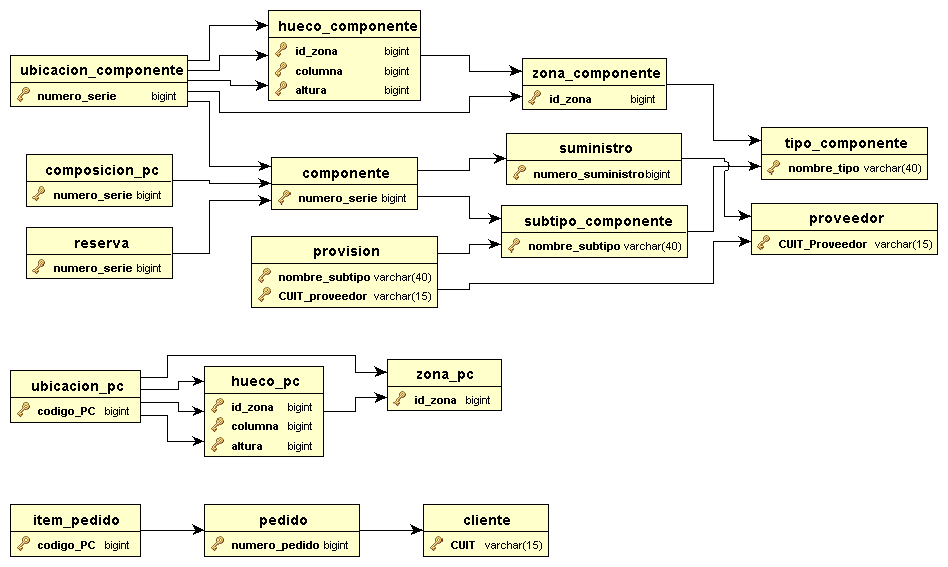
\includegraphics[scale=.5]{modelo_referencias.PNG}

	

	\subsection{ZONA\_PC}
		\subsubsection*{Atributos}
			\begin{itemize}
				\item id\_zona
				\item nombre\_configuracion
			\end{itemize}
		\subsubsection*{Claves candidatas}
			\begin{itemize}
				\item id\_zona
			\end{itemize}
		\subsubsection*{Clave primaria}
			\begin{itemize}
				\item id\_zona
			\end{itemize}
		\subsubsection*{Claves for�neas}
			\begin{itemize}
				\item nombre\_configuracion
			\end{itemize}
		\subsubsection*{Atributos que pueden tomar valores nulos}
			Ninguno
		
	\subsection{ZONA\_COMPONENTE}
		\subsubsection*{Atributos}
			\begin{itemize}
				\item id\_zona
				\item nombre\_tipo
			\end{itemize}
		\subsubsection*{Claves candidatas}
			\begin{itemize}
				\item id\_zona
			\end{itemize}
		\subsubsection*{Clave primaria}
			\begin{itemize}
				\item id\_zona
			\end{itemize}
		\subsubsection*{Claves for�neas}
			\begin{itemize}
				\item nombre\_tipo
			\end{itemize}
		\subsubsection*{Atributos que pueden tomar valores nulos}
			Ninguno
		
	\subsection{HUECO\_COMPONENTE}
		\subsubsection*{Atributos}
			\begin{itemize}
				\item id\_zona
				\item columna
				\item altura
			\end{itemize}
		\subsubsection*{Claves candidatas}
			\begin{itemize}
				\item (id\_zona, columna, altura)
			\end{itemize}
		\subsubsection*{Clave primaria}
			\begin{itemize}
				\item (id\_zona, columna, altura)
			\end{itemize}
		\subsubsection*{Claves for�neas}
			\begin{itemize}
				\item id\_zona
			\end{itemize}
		\subsubsection*{Atributos que pueden tomar valores nulos}
			Ninguno
		
	\subsection{HUECO\_PC}
		\subsubsection*{Atributos}
			\begin{itemize}
				\item id\_zona
				\item columna
				\item altura
			\end{itemize}
		\subsubsection*{Claves candidatas}
			\begin{itemize}
				\item (id\_zona, columna, altura)
			\end{itemize}
		\subsubsection*{Clave primaria}
			\begin{itemize}
				\item (id\_zona, columna, altura)
			\end{itemize}
		\subsubsection*{Claves for�neas}
			\begin{itemize}
				\item id\_zona
			\end{itemize}
		\subsubsection*{Atributos que pueden tomar valores nulos}
			Ninguno
		
	\subsection{UBICACI�N\_COMPONENTE}
		\subsubsection*{Atributos}
			\begin{itemize}
				\item n�mero\_serie
				\item id\_zona
				\item columna
				\item altura
			\end{itemize}
		\subsubsection*{Claves candidatas}
			\begin{itemize}
				\item n�mero\_serie
				\item (id\_zona, columna, altura)
			\end{itemize}
		\subsubsection*{Clave primaria}
			\begin{itemize}
				\item n�mero\_serie
			\end{itemize}
		\subsubsection*{Claves for�neas}
			\begin{itemize}
				\item n�mero\_serie
				\item id\_zona
				\item (id\_zona, columna, altura)
			\end{itemize}
		\subsubsection*{Atributos que pueden tomar valores nulos}
			Ninguno
		
	\subsection{COMPONENTE}
		\subsubsection*{Atributos}
			\begin{itemize}
				\item n�mero\_serie
				\item nombre\_subtipo
				\item n�mero\_suministro
				\item fecha\_llegada
				\item descripci�n
				\item estado
			\end{itemize}
		\subsubsection*{Claves candidatas}
			\begin{itemize}
				\item n�mero\_serie
			\end{itemize}
		\subsubsection*{Clave primaria}
			\begin{itemize}
				\item n�mero\_serie
			\end{itemize}
		\subsubsection*{Claves for�neas}
			\begin{itemize}
				\item nombre\_subtipo
				\item n�mero\_suministro
			\end{itemize}
		\subsubsection*{Atributos que pueden tomar valores nulos}
			\begin{itemize}
				\item fecha\_llegada
				\item descripci�n
			\end{itemize}
		
	\subsection{RESERVA}
		\subsubsection*{Atributos}
			\begin{itemize}
				\item n�mero\_serie
				\item n�mero\_ordenproduccion
			\end{itemize}
		\subsubsection*{Claves candidatas}
			\begin{itemize}
				\item n�mero\_serie
			\end{itemize}
		\subsubsection*{Clave primaria}
			\begin{itemize}
				\item n�mero\_serie
			\end{itemize}
		\subsubsection*{Claves for�neas}
			\begin{itemize}
				\item n�mero\_serie
				\item n�mero\_ordenproduccion
			\end{itemize}
		\subsubsection*{Atributos que pueden tomar valores nulos}
			Ninguno
		
	\subsection{COMPOSICI�N\_PC}
		\subsubsection*{Atributos}
			\begin{itemize}
				\item n�mero\_serie
				\item c�digo\_PC
			\end{itemize}
		\subsubsection*{Claves candidatas}
			\begin{itemize}
				\item n�mero\_serie
			\end{itemize}
		\subsubsection*{Clave primaria}
			\begin{itemize}
				\item n�mero\_serie
			\end{itemize}
		\subsubsection*{Claves for�neas}
			\begin{itemize}
				\item n�mero\_serie
				\item c�digo\_PC
			\end{itemize}
		\subsubsection*{Atributos que pueden tomar valores nulos}
			Ninguno
		
	\subsection{SUBTIPO\_COMPONENTE}
		\subsubsection*{Atributos}
			\begin{itemize}
				\item nombre\_subtipo
				\item descripci�n
				\item nombre\_tipo
				\item stock\_minimo
			\end{itemize}
		\subsubsection*{Claves candidatas}
			\begin{itemize}
				\item nombre\_subtipo
			\end{itemize}
		\subsubsection*{Clave primaria}
			\begin{itemize}
				\item nombre\_subtipo
			\end{itemize}
		\subsubsection*{Claves for�neas}
			\begin{itemize}
				\item nombre\_tipo
			\end{itemize}
		\subsubsection*{Atributos que pueden tomar valores nulos}
			\begin{itemize}
				\item descripcion
				\item stock\_minimo
			\end{itemize}
		
	\subsection{TIPO\_COMPONENTE}
		\subsubsection*{Atributos}
			\begin{itemize}
				\item nombre\_tipo
				\item descripci�n
			\end{itemize}
		\subsubsection*{Claves candidatas}
			\begin{itemize}
				\item nombre\_tipo
			\end{itemize}
		\subsubsection*{Clave primaria}
			\begin{itemize}
				\item nombre\_tipo
			\end{itemize}
		\subsubsection*{Claves for�neas}
			No hay
		\subsubsection*{Atributos que pueden tomar valores nulos}
			\begin{itemize}
				\item descripci�n
			\end{itemize}
			Ninguno
		
	\subsection{SUMINISTRO}
		\subsubsection*{Atributos}
			\begin{itemize}
				\item n�mero\_suministro
				\item CUIT\_proveedor
				\item impreso
			\end{itemize}
		\subsubsection*{Claves candidatas}
			\begin{itemize}
				\item n�mero\_suministro
			\end{itemize}
		\subsubsection*{Clave primaria}
			\begin{itemize}
				\item n�mero\_suministro
			\end{itemize}
		\subsubsection*{Claves for�neas}
			\begin{itemize}
				\item CUIT\_proveedor
			\end{itemize}
		\subsubsection*{Atributos que pueden tomar valores nulos}
			Ninguno
		
	\subsection{PROVEEDOR}
		\subsubsection*{Atributos}
			\begin{itemize}
				\item CUIT\_proveedor
				\item Nombre
				\item Direcci�n
				\item Tel�fono
				\item FAX
				\item email
			\end{itemize}
		\subsubsection*{Claves candidatas}
			\begin{itemize}
				\item CUIT\_proveedor
			\end{itemize}
		\subsubsection*{Clave primaria}
			\begin{itemize}
				\item CUIT\_proveedor
			\end{itemize}
		\subsubsection*{Claves for�neas}
			No hay
		\subsubsection*{Atributos que pueden tomar valores nulos}
			\begin{itemize}
				\item Nombre
				\item Direcci�n
				\item Tel�fono
				\item FAX
				\item email
			\end{itemize}
		
	\subsection{PROVISI�N}
		\subsubsection*{Atributos}
			\begin{itemize}
				\item nombre\_subtipo
				\item CUIT\_proveedor
				\item precio\_unitario
			\end{itemize}
		\subsubsection*{Claves candidatas}
			\begin{itemize}
				\item (nombre\_subtipo, CUIT\_proveedor)
			\end{itemize}
		\subsubsection*{Clave primaria}
			\begin{itemize}
				\item (nombre\_subtipo, CUIT\_proveedor)
			\end{itemize}
		\subsubsection*{Claves for�neas}
			\begin{itemize}
				\item nombre\_subtipo
				\item CUIT\_proveedor
			\end{itemize}
		\subsubsection*{Atributos que pueden tomar valores nulos}
			\begin{itemize}
				\item precio\_unitario
			\end{itemize}
		
	\subsection{UBICACI�N\_PC}
		\subsubsection*{Atributos}
			\begin{itemize}
				\item c�digo\_PC
				\item id\_zona
				\item columna
				\item altura
			\end{itemize}
		\subsubsection*{Claves candidatas}
			\begin{itemize}
				\item c�digo\_PC
				\item (id\_zona, columna, altura)
			\end{itemize}
		\subsubsection*{Clave primaria}
			\begin{itemize}
				\item c�digo\_PC
			\end{itemize}
		\subsubsection*{Claves for�neas}
			\begin{itemize}
				\item c�digo\_PC
				\item id\_zona
				\item (id\_zona, columna, altura)
			\end{itemize}
		\subsubsection*{Atributos que pueden tomar valores nulos}
			Ninguno
		
	\subsection{PEDIDO}
		\subsubsection*{Atributos}
			\begin{itemize}
				\item n�mero\_pedido
				\item CUIT\_cliente
				\item fecha\_pedido
				\item direcci�n\_entrega
			\end{itemize}
		\subsubsection*{Claves candidatas}
			\begin{itemize}
				\item n�mero\_pedido
			\end{itemize}
		\subsubsection*{Clave primaria}
			\begin{itemize}
				\item n�mero\_pedido
			\end{itemize}
		\subsubsection*{Claves for�neas}
			\begin{itemize}
				\item CUIT\_cliente
			\end{itemize}
		\subsubsection*{Atributos que pueden tomar valores nulos}
			\begin{itemize}
				\item fecha\_pedido
				\item direcci�n\_entrega
			\end{itemize}
		
	\subsection{ITEM\_PEDIDO}
		\subsubsection*{Atributos}
			\begin{itemize}
				\item c�digo\_PC
				\item n�mero\_pedido
			\end{itemize}
		\subsubsection*{Claves candidatas}
			\begin{itemize}
				\item c�digo\_PC
			\end{itemize}
		\subsubsection*{Clave primaria}
			\begin{itemize}
				\item c�digo\_PC
			\end{itemize}
		\subsubsection*{Claves for�neas}
			\begin{itemize}
				\item n�mero\_pedido			
				\item c�digo\_PC
			\end{itemize}
		\subsubsection*{Atributos que pueden tomar valores nulos}
			Ninguno
		
	\subsection{CLIENTE}
		\subsubsection*{Atributos}
			\begin{itemize}
				\item CUIT\_cliente
				\item Nombre
				\item Direcci�n
				\item Tel�fono
				\item FAX
				\item email
			\end{itemize}
		\subsubsection*{Claves candidatas}
			\begin{itemize}
				\item CUIT\_cliente
			\end{itemize}
		\subsubsection*{Clave primaria}
			\begin{itemize}
				\item CUIT\_cliente
			\end{itemize}
		\subsubsection*{Claves for�neas}
			No hay
		\subsubsection*{Atributos que pueden tomar valores nulos}
			\begin{itemize}
				\item Nombre
				\item Direcci�n
				\item Tel�fono
				\item FAX
				\item email
			\end{itemize}
	
	


		
	\subsection{Sentencias DDL}		

	
	

\clearpage	
\section{Alternativas en la transformaci�n de MER al modelo de tablas}		
	\paragraph{Uso de relaci\'on general para zonas contra relaciones solo para zonas especificas (PC y componentes). \\}
		La primera alternativa nos permite tener un id \'unico por zona. 
		Esto pod\'ia llegar a ser conveniente en caso de que se necesitar\'an hacer consultas para todas las zonas de los dos tipos. 
		Como estas consultas no son necesarias, el uso de esta relaci\'on es redundante. 
		Las consultas se hacen unicamente sobre zonas de PCs y zonas de Componentes.
		
	\paragraph{Uso de CUIT como clave primaria de proveedores y clientes contra una clave primaria numerica m\'as peque�a.\\}
		La segunda alternativa parec\'ia ser una buena opci\'on ya que utilizar las consultas usando el CUIT pueden resultar m\'as costosas que consultas en las cuales se comparen numeros cortos. 
		De todas formas, nos inclinamos por la primera opci\'on porque encontramos m\'as de un requisito que justificaba el uso del CUIT como clave primaria. Algunos de estos requisitos son los siguientes:
			\begin{itemize}
				\item \textit{Si el usuario desea dar de baja a un cliente existente, comunicar\'a al sistema el CUIT del cliente en cuesti\'on.}
				
				\item \textit{Los pedidos de los clientes ser\'an dados de alta en el sistema. Los datos b\'asicos del pedido son: Fecha del pedido, el CUIT del cliente, el nombre del cliente y la direcci\'on de entrega}		
			\end{itemize}




\end{document}